
\chapter{Safe and near optimal controller synthesis}

% proposal
\label{ch:proposal}
In this part, we choose as a case of study an \emph{Hybrid Solar Water
Heating}, because this system link up important condition to implement the
methodology described in this work. Firstly we have agents, who interact with 
the system, adding uncontrollables modes of operations also some controllable
variables in the system that allow to model as stochastic hybrid game.

The first part is about mathematical modelling using heat transfer
theory and fluids dynamics to get temperature dinamics and then 
to define the parameters that determine the system with some
assumptions to facilate the analysis.

\clearpage
\section{Solar Water Heating Case study}

\textbf{Setup system}:

\begin{figure}[!hbt]


\tikzset{every picture/.style={line width=0.75pt}} %set default line width to 0.75pt        

\begin{tikzpicture}[x=0.75pt,y=0.75pt,yscale=-1,xscale=1]
%uncomment if require: \path (0,300); %set diagram left start at 0, and has height of 300

%Rounded Rect [id:dp3454362135099034] 
\draw   (203,113.4) .. controls (203,105.45) and (209.45,99) .. (217.4,99) -- (282.1,99) .. controls (290.05,99) and (296.5,105.45) .. (296.5,113.4) -- (296.5,156.6) .. controls (296.5,164.55) and (290.05,171) .. (282.1,171) -- (217.4,171) .. controls (209.45,171) and (203,164.55) .. (203,156.6) -- cycle ;
%Straight Lines [id:da8670184653139519] 
\draw    (232.5,128) -- (175.5,128.97) ;
\draw [shift={(173.5,129)}, rotate = 359.03] [color={rgb, 255:red, 0; green, 0; blue, 0 }  ][line width=0.75]    (10.93,-3.29) .. controls (6.95,-1.4) and (3.31,-0.3) .. (0,0) .. controls (3.31,0.3) and (6.95,1.4) .. (10.93,3.29)   ;
%Image [id:dp1573774251550818] 
\draw (329.75,151.88) node  {\includegraphics[width=391.13pt,height=232.5pt]{content/sources/5.png}};
%Straight Lines [id:da756821456781489] 
\draw    (368.5,118.55) -- (450.5,117.57) ;
\draw [shift={(452.5,117.55)}, rotate = 539.3199999999999] [color={rgb, 255:red, 0; green, 0; blue, 0 }  ][line width=0.75]    (10.93,-3.29) .. controls (6.95,-1.4) and (3.31,-0.3) .. (0,0) .. controls (3.31,0.3) and (6.95,1.4) .. (10.93,3.29)   ;
%Straight Lines [id:da9580285561891552] 
\draw    (228.5,102.22) -- (302.5,101.24) ;
\draw [shift={(304.5,101.22)}, rotate = 539.25] [color={rgb, 255:red, 0; green, 0; blue, 0 }  ][line width=0.75]    (10.93,-3.29) .. controls (6.95,-1.4) and (3.31,-0.3) .. (0,0) .. controls (3.31,0.3) and (6.95,1.4) .. (10.93,3.29)   ;
%Straight Lines [id:da9281060785864365] 
\draw    (413,77.89) -- (413,107.89) ;
\draw [shift={(413,109.89)}, rotate = 270] [color={rgb, 255:red, 0; green, 0; blue, 0 }  ][line width=0.75]    (10.93,-3.29) .. controls (6.95,-1.4) and (3.31,-0.3) .. (0,0) .. controls (3.31,0.3) and (6.95,1.4) .. (10.93,3.29)   ;
%Straight Lines [id:da47053369422446445] 
\draw    (261.5,79.22) -- (294.5,79.22) ;
\draw [shift={(296.5,79.22)}, rotate = 180] [color={rgb, 255:red, 0; green, 0; blue, 0 }  ][line width=0.75]    (10.93,-3.29) .. controls (6.95,-1.4) and (3.31,-0.3) .. (0,0) .. controls (3.31,0.3) and (6.95,1.4) .. (10.93,3.29)   ;
%Shape: Circle [id:dp11314595015500317] 
\draw  [color={rgb, 255:red, 0; green, 0; blue, 0 }  ,draw opacity=1 ][fill={rgb, 255:red, 155; green, 155; blue, 155 }  ,fill opacity=1 ] (532.5,92.75) .. controls (532.5,88.19) and (536.19,84.5) .. (540.75,84.5) .. controls (545.31,84.5) and (549,88.19) .. (549,92.75) .. controls (549,97.31) and (545.31,101) .. (540.75,101) .. controls (536.19,101) and (532.5,97.31) .. (532.5,92.75) -- cycle ;
%Shape: Rectangle [id:dp7839106216211671] 
\draw  [color={rgb, 255:red, 0; green, 0; blue, 0 }  ,draw opacity=1 ][fill={rgb, 255:red, 0; green, 0; blue, 0 }  ,fill opacity=0.25 ] (344.33,136.55) -- (352.33,136.55) -- (352.33,174.55) -- (344.33,174.55) -- cycle ;
%Straight Lines [id:da12515710435460292] 
\draw    (375.67,136.55) -- (321,136.22) ;
%Straight Lines [id:da47364591531914657] 
\draw [color={rgb, 255:red, 208; green, 2; blue, 27 }  ,draw opacity=1 ][line width=1.5]    (383,57.89) -- (417,57.89) ;
%Straight Lines [id:da715354649143032] 
\draw  [dash pattern={on 4.5pt off 4.5pt}]  (374.33,104.55) -- (320.33,103.89) ;
%Straight Lines [id:da06846603339970381] 
\draw  [dash pattern={on 4.5pt off 4.5pt}]  (375.67,75.89) -- (321.67,75.22) ;
%Straight Lines [id:da8948879575945841] 
\draw    (340.33,223.89) -- (339.68,147.22) ;
\draw [shift={(339.67,145.22)}, rotate = 449.51] [color={rgb, 255:red, 0; green, 0; blue, 0 }  ][line width=0.75]    (10.93,-3.29) .. controls (6.95,-1.4) and (3.31,-0.3) .. (0,0) .. controls (3.31,0.3) and (6.95,1.4) .. (10.93,3.29)   ;

% Text Node
\draw (455,133) node    {$kA_{t}( T_{c} -T_{e})$};
% Text Node
\draw (193,97) node    {$A_{c} I_{e}$};
% Text Node
\draw (469.33,90) node    {$v\dot{m}( T_{c} -T_{i})$};
% Text Node
\draw (348.33,120) node    {$T_{c} ,V_{c}$};
% Text Node
\draw (568,89) node    {$T_{e}$};
% Text Node
\draw (539,278) node    {$T_{i}$};
% Text Node
\draw (281.33,66.67) node    {$P_{a} =c_{3} r$};
% Text Node
\draw (540,217) node    {$T_{c}$};
% Text Node
\draw (382.67,126.33) node [anchor=north west][inner sep=0.75pt]   [align=left] {1};
% Text Node
\draw (382,93) node [anchor=north west][inner sep=0.75pt]   [align=left] {2};
% Text Node
\draw (382,57.33) node [anchor=north west][inner sep=0.75pt]   [align=left] {3};
% Text Node
\draw (272.67,213.73) node [anchor=north west][inner sep=0.75pt]    {$\frac{dV_{c}( t)}{dt} =pV_{min} -V_{c}( t)$};


\end{tikzpicture}

\caption{Solar Water Heating diagram}
\end{figure}

% equation description
The energy inside of the container is calculated as a control volumen, an abstract
region which experiment power input and output, doing a energy balance is obtained
the dynamical either volumen or temperature as described in \ref{energy-balance}
and \ref{volume-balance}.

\begin{equation} 
    \factorheat\mcont(t)\frac{d}{dt}\tcont =  A_c\irradiance + \haux - v\factorheat \flowin (\tcont-\tin) -   k_c A_t (\tcont-\tenv) + rQ
    \label{energy-balance}
\end{equation}

\begin{equation}
    \frac{d}{dt}\mcont(t) =  \rho \frac{d}{dt}\vcont = \rho (pV_{min} - \vcont); \quad
    \label{volume-balance}
\end{equation}

% table 
\begin{table}[hbt!]
\begin{tabular}{ |p{2cm}||p{6cm}|p{2cm}|p{2cm}|  }
    \hline
    \multicolumn{4}{|c|}{States} \\
    \hline
    Variable& Description &Initial Value&Units\\    
    \hline    
    E & Energy consumption  & 0.0 & \si{\joule} \\
    V & Container Volumen  & 0.13 &\si{\metre^3}\\
    T & Container Temperature & 50.0 & \si{\degreeCelsius}  \\            
    \hline
    \multicolumn{4}{|c|}{Constants} \\
    \hline    
    Variable& Description & Value & Units\\        
    \hline
    \factorheat & The factor heat of the water in   & 4186&\si{\joule\per\degreeCelsius\per\kilogram}\\
    \flowin & Mass flow rate input/output  & 0.1  &\si{\kilogram\per\second}\\
    \mcont & the mass of the container in & 100 & \si{\kilogram} \\    
    $A_c$ & Area of colector in & 1 & \si{\metre^2} \\
    $A_t$ & Area of total of surface in & 5.56 & \si{\metre^2} \\
    $k_c$ & Conduction coeficient & 16 & \si{\watt\per\metre\per\degreeCelsius} \\
    $\haux$ & Auxiliary heat power in & 1000 & \si{\watt} \\    
    \hline
    \multicolumn{4}{|c|}{Input values} \\
    \hline    
    Variable& Description &  \multicolumn{2}{|c|}{Space values}\\
    \hline
    $v$ & Controllable action to release water & \multicolumn{2}{|c|}{$\left\lbrace 0,1 \right\rbrace$} \\
    \hline
    $r$ & Controllable action to heat & \multicolumn{2}{|c|}{$\left\lbrace 0,1 \right\rbrace$}\\
    \hline
    $p$ & Uncontrollable action to change capacity water & \multicolumn{2}{|c|}{$\left\lbrace 1,2,3 \right\rbrace$}\\
    \hline         
    \multicolumn{4}{|c|}{Disturbances} \\
    \hline
    Variable& Description & Range&Units\\        
    \hline
    $\tin$ & the temperature of water input/output in & $[20-25]$ & \si{\degreeCelsius} \\
    $\irradiance$ & the irradiance in & $[0-920]$ & \si{\watt\per\square\metre}    \\
    $\tenv$ & the outside temperature in & $[0-16.5]$ & \si{\degreeCelsius} \\
    \hline
\end{tabular}
\caption{Parameter values.}
\label{data-table}
\end{table}

\clearpage

\textbf{Hybrid Solar Water Heating as a Sthocastic Hybrid Game}.
The hybrid solar water heating scenario with 12 modes of operations is
defined  like this: $\mathcal{G}_{n,m} = (\mathcal{C,U,X,F},\delta)$, 
where the controller $\mathcal{C}$ has a finite set of controllable modes,
given by resistance state ${r \in \mathbb{B}}$ and piston position $p \in 
\left\lbrace1,2,3\right\rbrace $. The environment $\mathcal{U}$ has a finite  
set of uncontrollable modes $v \in \mathbb{B} $, that means the valve state 
for opening/closing water aperture. We assume that $\mathcal{U}$ given
$\delta$ can switch among modes with equal probability at every period. 
The state variables in $\mathcal{X}$ are given by $\left\lbrace
T,E,V \right\rbrace $, container temperature, energy used and container volumen
respectively.

Given the container temparature and volume, a controllable modes $r \in \mathbb{B}$
and $p \in \left\lbrace1,2,3\right\rbrace $ and uncontrollable mode
$v \in \mathbb{B} $ and a time delay $\tau$.

\begin{equation}
    \begin{aligned}
\frac{d}{dt}\tcont = \frac{1}{V(t)} [ -\constone(\tcont-\tenv)
- p \consttwo(\tcont-\tin) \\
- f \constthree(pV_{min} - \vcont)(\tcont-\tin)
+ \constfour\irradiance+ 
r \constfive ]
    \end{aligned}
\label{temperature-equation}
\end{equation}

\begin{equation}
\frac{d}{dt}\vcont = pV_{min} - \vcont; \quad
\label{volume-equation}
\end{equation}

\begin{equation} 
\frac{d}{dt}E_{used} =  r \constthree ;
\label{Energy-equation}
\end{equation}

The equation \ref{temperature-equation} has some constants $\left\lbrace 
\constone, \consttwo, \constthree, \constfour \right\rbrace $ this
parameters are computed with the parameteres defines in table \ref{data-table} for specific Hybrid Solar Water Heating
are equal to $\left\lbrace 2.44e^{-5},  4.77e^{-6}
, 0.0024, 0.01  \right\rbrace$ respectively.

\clearpage

\section{Simulations and Results}
%\subsection{Solaris Data and prediction data}
\textbf{Solaris Data and prediction data}
The Figure environment "floats" to find an optimal position on the page. When you begin a figure, you can use the options [htbp!] to specify whether the figure should go "here", the "top" of this page, the "bottom" of this page, or a special "page" reserved for floats. LaTeX, in its infinite wisdom, will sometimes prevent you from putting a figure in an "ugly" place, but.


\begin{figure}[!hbt]
    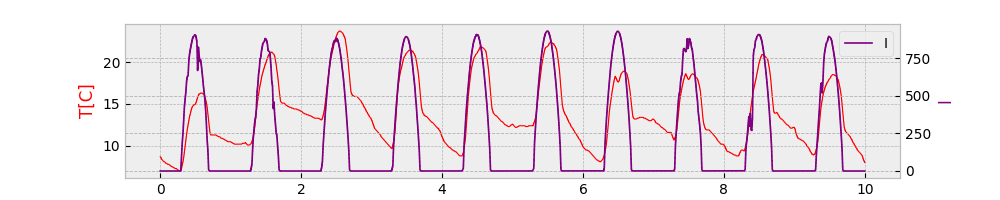
\includegraphics[width=1.2\linewidth]{images/solaris2}
    \captionof{figure}{An example image not including a Wombat}
\end{figure}

% \begin{minipage}{\linewidth}[!hbt]
%     \begin{center}  
%         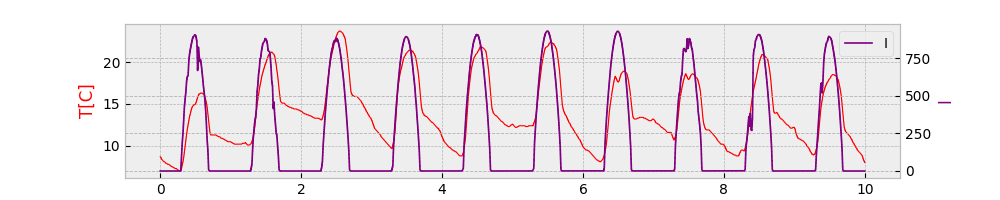
\includegraphics[width=1.2\linewidth]{images/solaris2}
%         \captionof{figure}{An example image not including a Wombat}
%     \end{center}
% \end{minipage}

\textbf{Data preparation}.
The Figure environment "floats" to find an optimal position on the page. When you begin a figure, you can use the options .

% \begin{figure}[!hbt]
%     \begin{center}
%     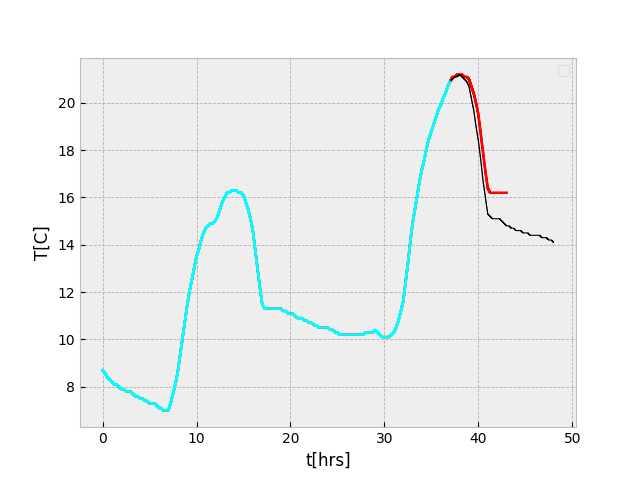
\includegraphics[width=0.8\linewidth]{images/prediction}
%     \captionof{figure}{An example of prediction using \textsc{arima} forecaster}
%     \end{center}
% \end{figure}

\begin{minipage}{\linewidth}
    \begin{center}
        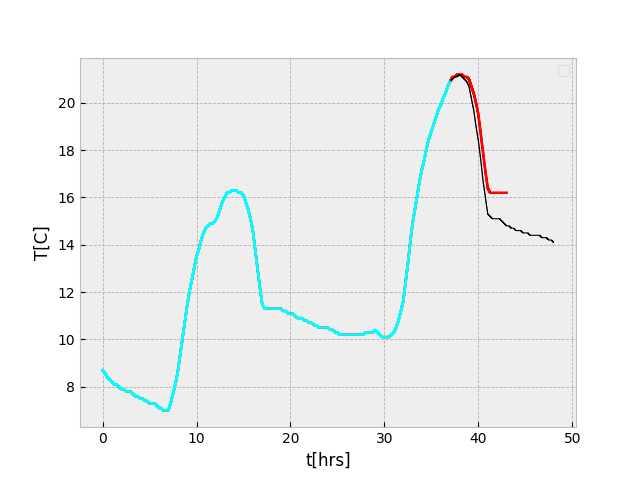
\includegraphics[width=0.8\linewidth]{images/prediction}
        \captionof{figure}{An example of prediction using \textsc{arima} forecaster}
    \end{center}
\end{minipage}

%\subsection{Experiments}
\textbf{Experiments}
[floor heating]
Regarding our experiments, we have two major components: a simulator 
written in  \textsc{Python} and a number of controllers, including 
the ones produced by \textsc{uppaal stratego}. The simulator implements
the solar water heating hybrid game $\mathcal{G}_{n,m}$. For our 
experiments, in the simulator we fix a time horizon \emph{H} of 75 minutes
with a period \emph{P} of 5 minutes. As in the real house, every 
15 minutes, the simulator outputs the current room temperatures \emph{T}
which are read by the controller. Subsequently, the controller inputs
the control valves \emph{V} which are used by the simulator for the
next 5 minutes. The house has a desired temperature $T^g$ and alpha
parameters which denotes the importance to optimize either target or 
energy consumption. Our goal is to optimize the comfort in the water 
consumption and also energy consumption as a cost function. To define 
this cost function subject to controller (strategy) $\sigma$ and 
$\mathcal{G}_{n,m}$ of the form $\pi = \gamma_0 \xrightarrow{t_{1}} 
\gamma_1 \xrightarrow{t_{2}} ... \xrightarrow{t_{k-1}} 
\gamma_{k-1} \xrightarrow{t_{k}} \gamma_{k}$ where $k = H/P$ is the 
number of control steps in the run $\pi$. Let $T_{i}(\gamma_j)$ denote
the container temperature $T_i$ at configuration $\gamma_j$. Then the 
const function is defined by

\begin{equation}
    \begin{aligned}
        dist(\pi) = \alpha(E) + (1-\alpha)(T-T_g)
    \end{aligned}
\end{equation}

In our experiments, we evaluate a number of different controllers. The 
simulator uses the distance function dist to compare the different
controllers.

\textbf{Controllers}. In the following we introduce a number of controllers
which we use in out experiments. We present the current controller operating
in the house, two controllers proposed by engineers and the controllers 
synthetized using online synthesis and \textsc{uppaal-stratego}.

\emph{Bang-Bang Controller}. The bang-bang controller is currently running
in the physical house and after each reading of container temperature $T$,
it simply switch the resistor $ON$ of container where $T < T^g$ and leaves 
the reaiming switch $OFF$.

\emph{Greedy controller}


\emph{Safe Controller with Patterns}. 
The Figure environment "floats" to find an optimal position on the page. When you begin a figure, you can use the options [htbp!] to specify whether the figure should go "here", the "top" of this page, the "bottom" of this page, or a special "page" reserved for floats. LaTeX, in its infinite wisdom, will sometimes prevent you from putting a figure in an "ugly" place, but you can (sort of) override its decision using the "!" option. When you haven't used any option, the environment assumes that you provided [tbp], and it's choosing to put the figure at the top of the page, above where your section goes.

\emph{Statego Online Controller}.
The Figure environment "floats" to find an optimal position on the page. When you begin a figure, you can use the options [htbp!] to specify whether the figure should go "here", the "top" of this page, the "bottom" of this page, or a special "page" reserved for floats. LaTeX, in its infinite wisdom, will sometimes prevent you from putting a figure in an "ugly" place, but you can (sort of) override its decision using the "!" option. When you haven't used any option, the environment assumes that you provided [tbp], and it's choosing to put the figure at the top of the page, above where your section goes.
\begin{minipage}{\linewidth}
    \begin{center}
        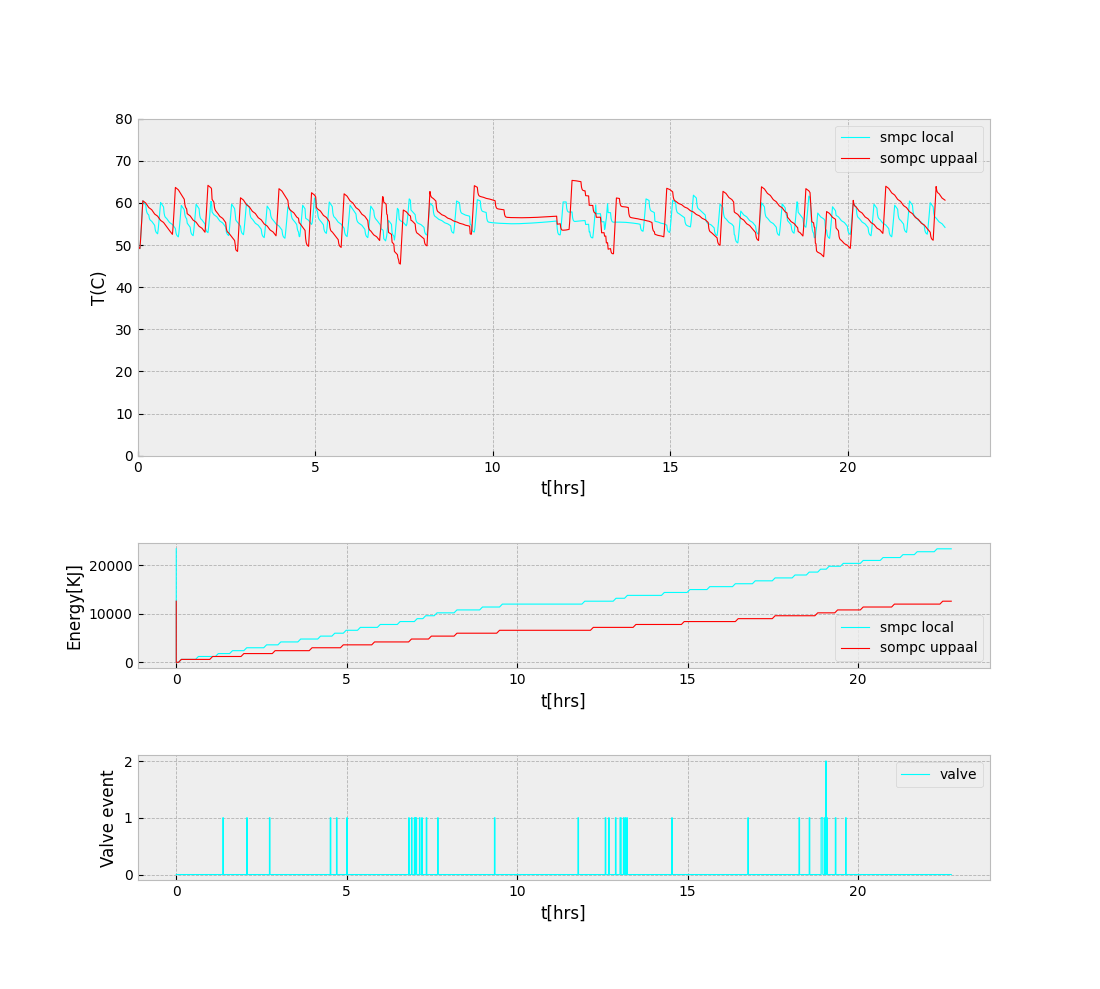
\includegraphics[width=1.0\linewidth]{images/Simulation}
        \captionof{figure}{An example image not including a Wombat}
    \end{center}
\end{minipage}

\emph{Safe and Near Optimal Controller}.


\textbf{Evaluation Scenarios}

\textbf{Controller Evaluation}

